\documentclass[letterpaper,12pt]{article}
\usepackage{array}
\usepackage{threeparttable}
\usepackage{geometry}
\geometry{letterpaper,tmargin=1in,bmargin=1in,lmargin=1.25in,rmargin=1.25in}
\usepackage{fancyhdr,lastpage}
\pagestyle{fancy}
\lhead{}
\chead{}
\rhead{}
\lfoot{}
\cfoot{}
\rfoot{\footnotesize\textsl{Page \thepage\ of 2}}
\renewcommand\headrulewidth{0pt}
\renewcommand\footrulewidth{0pt}
\usepackage[format=hang,font=normalsize,labelfont=bf]{caption}
\usepackage{listings}
\lstset{frame=single,
  language=Python,
  showstringspaces=false,
  columns=flexible,
  basicstyle={\small\ttfamily},
  numbers=none,
  breaklines=true,
  breakatwhitespace=true
  tabsize=3
}
\usepackage{amsmath}
\usepackage{amssymb}
\usepackage{amsthm}
\usepackage{harvard}
\usepackage{setspace}
\usepackage{float,color}
\usepackage[pdftex]{graphicx}
\usepackage{hyperref}
\hypersetup{colorlinks,linkcolor=red,urlcolor=blue}
\theoremstyle{definition}
\newtheorem{theorem}{Theorem}
\newtheorem{acknowledgement}[theorem]{Acknowledgement}
\newtheorem{algorithm}[theorem]{Algorithm}
\newtheorem{axiom}[theorem]{Axiom}
\newtheorem{case}[theorem]{Case}
\newtheorem{claim}[theorem]{Claim}
\newtheorem{conclusion}[theorem]{Conclusion}
\newtheorem{condition}[theorem]{Condition}
\newtheorem{conjecture}[theorem]{Conjecture}
\newtheorem{corollary}[theorem]{Corollary}
\newtheorem{criterion}[theorem]{Criterion}
\newtheorem{definition}[theorem]{Definition}
\newtheorem{derivation}{Derivation} % Number derivations on their own
\newtheorem{example}[theorem]{Example}
\newtheorem{exercise}[theorem]{Exercise}
\newtheorem{lemma}[theorem]{Lemma}
\newtheorem{notation}[theorem]{Notation}
\newtheorem{problem}[theorem]{Problem}
\newtheorem{proposition}{Proposition} % Number propositions on their own
\newtheorem{remark}[theorem]{Remark}
\newtheorem{solution}[theorem]{Solution}
\newtheorem{summary}[theorem]{Summary}
%\numberwithin{equation}{section}
\bibliographystyle{aer}
\newcommand\ve{\varepsilon}
\newcommand\boldline{\arrayrulewidth{1pt}\hline}


\begin{document}

\begin{flushleft}
  \textbf{\large{Problem Set} 1} \\
  OSM Lab-Econ \\
  Sophia Mo
\end{flushleft}

\vspace{5mm}

\noindent\textbf{Problem 1}
The steady-state values are:\\
\begin{table}[htbp]
\begin{tabular}{ll}
Savings:&[ 0.01931255,  0.05841117]\\
Capital and Labor:&[ 0.07772372,  2.2       ]\\
Wage and Interest rate:&[ 0.20172474,  2.43304586]\\
Consumption:&[ 0.1824122,   0.20961442,  0.24087319]\\
\end{tabular}
\end{table}

\noindent\textbf{Problem 2}
The steady-state values when $\beta = 0.55$ are: \\
\begin{table}[htbp]
\begin{tabular}{ll}
Savings:&[ 0.02817696,  0.07686557] \\
Capital and Labor:&[ 0.10504253,  2.2       ] \\
Wage and Interest rate:&[ 0.22415231,  1.88636   ] \\
Consumption:&[ 0.19597535,  0.22861559,  0.26669216]\\
\end{tabular}
\end{table}
\\
When all households are more patient, $\bar{b}_2, \bar{b}_3$ both increase since consumption in future periods are more valuable for the households than before, resulting in their saving more today to further smooth consumption across periods.\\
\\
$\bar{K}$ increases because by market clearing, it is equal to the sum of $\bar{b}_2$ and $\bar{b}_3$; $\bar{L}$ remains unchanged because it is an exogenous variable.\\
\\
$\bar{w}$ increases and $\bar{r}$ decreases because $\frac{K}{L}$ increases. From firms' first order conditions, we know wage increases when capital-labor ratio increases, and interest rate decreases when capital labor ratio decrease (firms always optimize their capital-labor ratio according to prices).\\
\\
$\bar{c}_1, \bar{c}_2, \bar{c}_3$ all increase because income effect dominates intertemporal substitution effect--the increase in wage is much larger than the increase in households' savings for both periods.
\\
\\
\noindent\textbf{Problem 3}
Please see the python scipt for details of the time path. I choose T=30, and $b_{2,1}, b_{3,1}$ as required.
\\
\\
\noindent\textbf{Problem 4}
It only takes 3 periods for the aggregate capital stock to be within 0.0001 of the steady-state value, assuming $\beta = 0.442$. So $T=3$ if we label the first period 1. I also found the second t(=7) such that the capital stock is within 0.0001 of the steady-state value.
\begin{center}
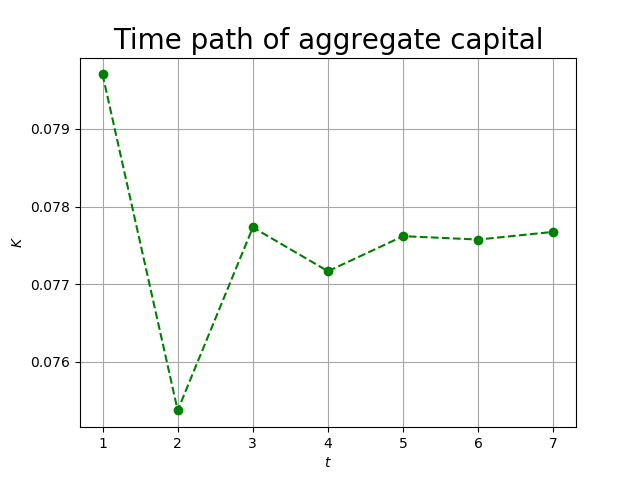
\includegraphics[scale=0.4]{/Users/Sophia/Desktop/Bootcamp2017/Econ/wk1_hw/images/kplot1}
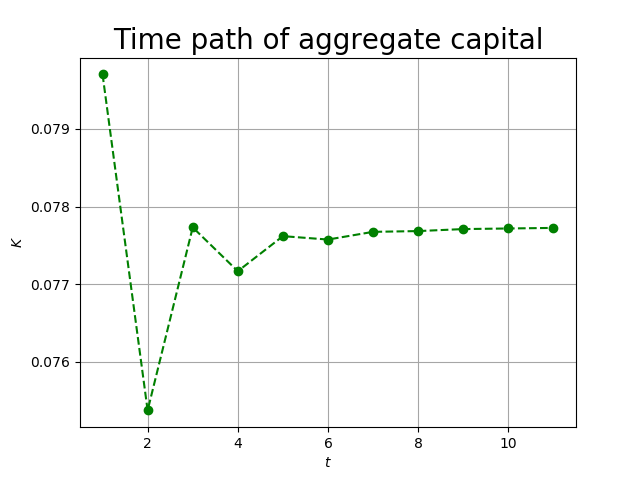
\includegraphics[scale=0.4]{/Users/Sophia/Desktop/Bootcamp2017/Econ/wk1_hw/images/kplot2}
\end{center}
\end{document}
